\section*{Method}
\label{Method}
%
In order to know whether or not the BTL model can be applied to the data shown in \autoref{tab:data}, it is first necessary to check for transitivity in the data. In other words how reliable and consistent the data is. The cumulative preference matrix is a pooled data matrix meaning it contains data from all the participants deemed sufficiently consistent. This is typically done using a $\chi^{2}-test$. Now a problem could arise because it is unknown whether the pooled subjects have shown an opposite decision behaviour (eg. chosen pleasant where others chose unpleasant) or not. If that is the case, then the preference matrix becomes inconsistent. Before it is possible to do the transitivity check, it is necessary to calculate the probability of a stimulus being rated as unpleasant. See \autoref{eg:probability}.

\begin{equation}
p = \frac{freq}{n}
\end{equation}

Here \textit{freq} is the frequency that a sound has been rated unpleasant (the pooled preference matrix, \autoref{tab:data}) and \textit{n} is the amount of test subjects. Thereafter it is needed to check every combination of the stimuli for transitivity violations. There are no set rules but a rough estimate of when the probabilistic choice models holds is shown in \autoref{tab:trans_violations}:

% Please add the following required packages to your document preamble:
% \usepackage{booktabs}
\begin{table}[H]
\centering
\begin{tabular}{@{}ll@{}}
\toprule
Transitivity violations                                    & Expected                                      \\ \midrule
None or few SST violations                                 & BTL may fit                                   \\
Some SST violations and few MST violations                 & Preference-tree might fit (Not BTL)            \\
Considerable SST and MST but few WST violations & Possible to rank order (no model will fit) \\ \bottomrule
\end{tabular}
\caption{General estimates of the outcome of probabilistic choice models considering the amount of weak (WST), moderate (MST) and stong (SST) transitivity violations}
\label{tab:trans_violations}
\end{table}

Consider three stimuli: \textit{a}, \textit{b}, and \textit{c}. If it is observed that $p_{ab} \geq 0.05$ and $p_{ab} \geq 0.05$, in other words if the probability of \textit{a} being rated as more unpleasant compared to \textit{b} and \textit{b} more unpleasant compared to \textit{c}. Then Weak Stochastic Transitivity (WST) holds when $p_{ac} \geq 0.05$. It is considered a WST violation if $p_{ac} < 0.05$. The same logic applies to MST and SST. If $p_{ac}$ is bigger than or equal to the minimum value in $p_{ab}$ and $p_{bc}$, MST holds( $p_{ac}\geq min(p_{ab};p_{bc}$). It is a violation if not. For SST, $p_{ac}$ is compared to the maximum value of both $p_{ab}$ and $p_{bc}$. If $p_{ac}$ is not bigger or equal to values, it counts as an SST (violation if $p_{ac}< max(p_{ab};p_{bc}$.)
 
Luckily, with the help of Matlab it is not needed to perform every single comparison by hand. A loop was written which identified the number of WST, MST and SST violations. See \autoref{fig:loop}.

\begin{figure}[H]
\centering
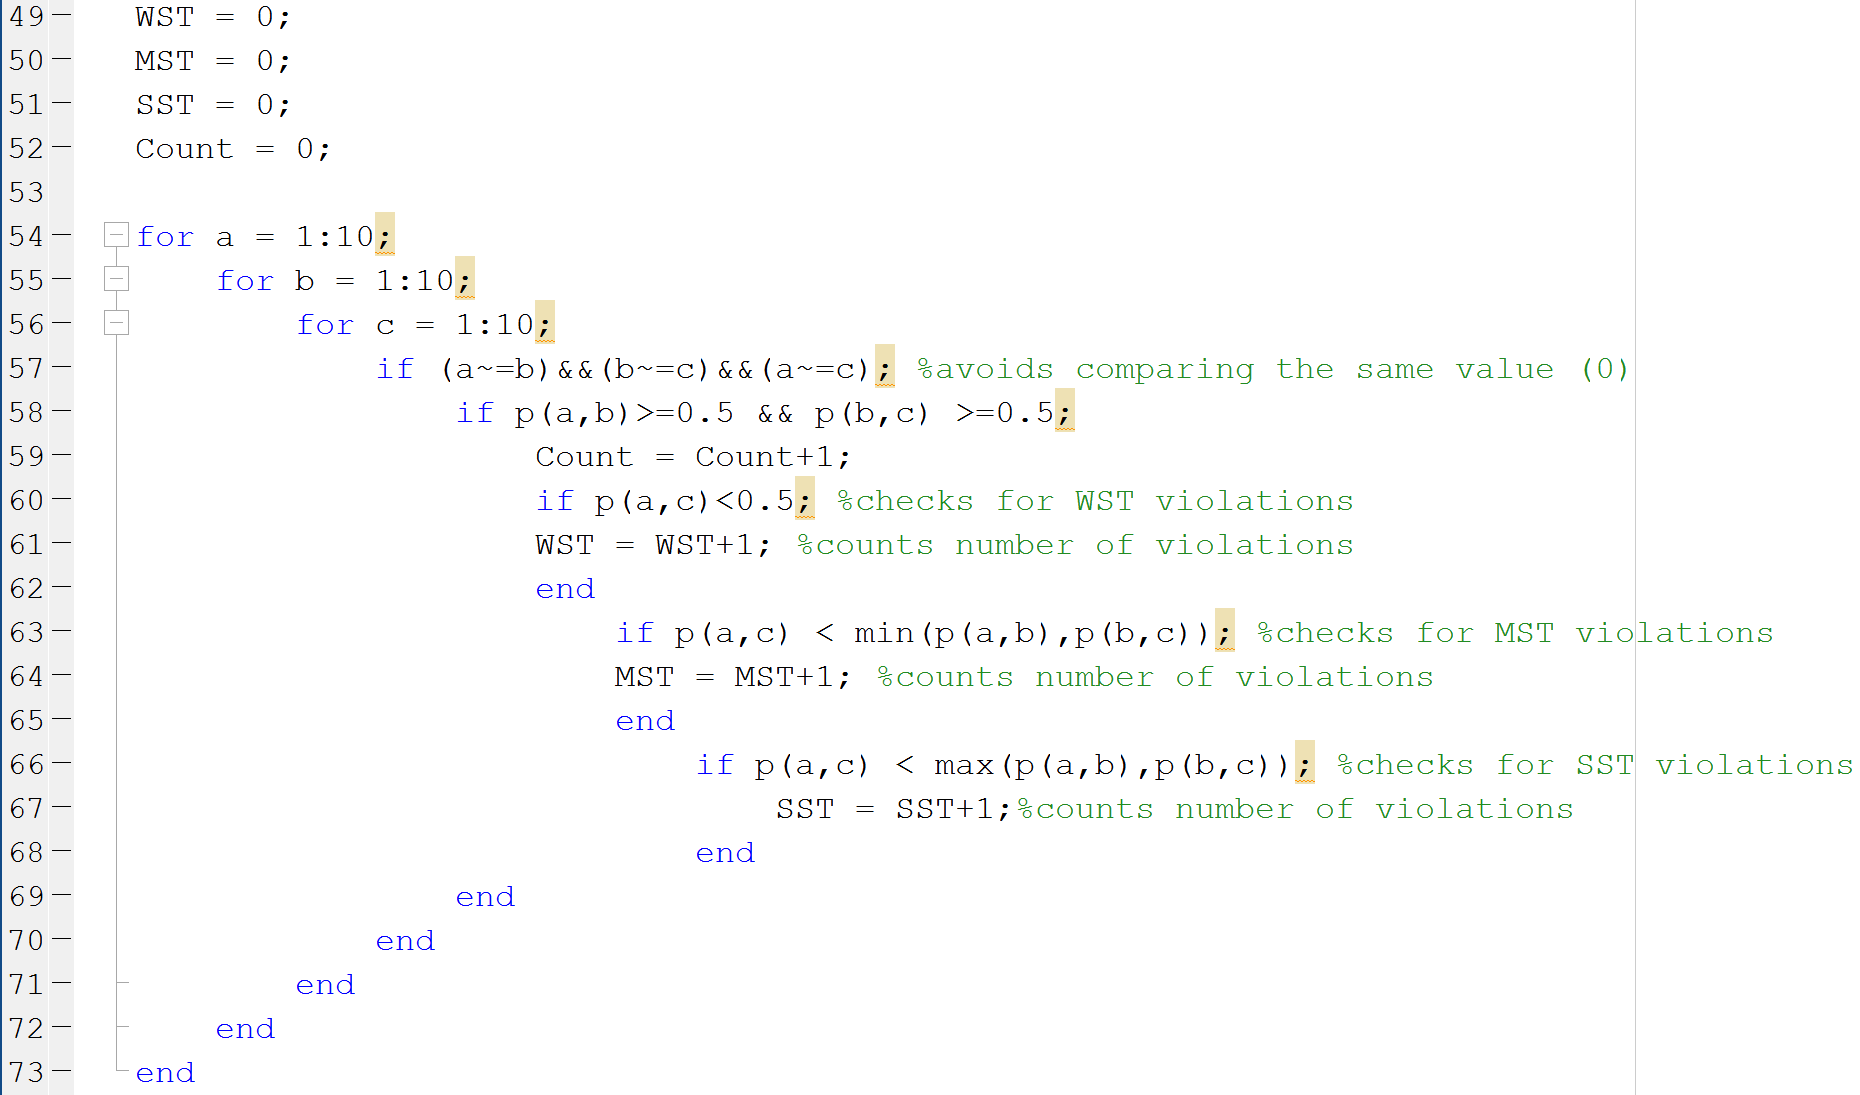
\includegraphics[width = \textwidth]{Figure/loop.png} 
\caption{Loop used to calculate WST, MST and SST violations}
\label{fig:loop}
\end{figure}



The same goes for the likelihood estimation. The  fOptiPt.m Matlab function has been developed for this purpose. The function requires two mandatory input, \textit{M} and \textit{A}, where \textit{M} is the paired comparison matrix shown in \autoref{tab:data}, and \textit{A} is a cell array with length corresponding to the number of stimuli. Further there is an optional input, \textit{s}, which denotes the starting values for the estimation routine. The search algorithm starts at $\frac{1}{k}$ for each parameter value, where \textit{k} is the number of parameters, if \textit{s} is not specified. In this case \textit{s} is not specified.


